\documentclass{article}

% Language setting
% Replace `english' with e.g. `spanish' to change the document language
\usepackage[english]{babel}

% Set page size and margins
% Replace `letterpaper' with `a4paper' for UK/EU standard size
\usepackage[a4paper,top=2cm,bottom=2cm,left=3cm,right=3cm,marginparwidth=1.75cm]{geometry}

% Useful packages
\usepackage{amsmath}
\usepackage{graphicx}
\usepackage[colorlinks=true, allcolors=blue]{hyperref}
\usepackage{xcolor}
\usepackage{listings}
\usepackage{multicol}
\colorlet{mygray}{black!30}
\colorlet{mygreen}{green!60!blue}
\colorlet{mymauve}{red!60!blue}



\lstdefinelanguage{makefile}{
otherkeywords={.SUFFIXES},
morekeywords={SUFFIX, CPP_,},
moredelim=[is][\color{mbleu}]{/*}{*/},
style=global,%
morecomment=[l][commentstyle]{\#},%
emphstyle={\color{vimvert}},%
moredelim=[s][\color{vimvert}]{\$(}{)}%
}

\lstdefinelanguage{cpp}{
  backgroundcolor=\color{gray!10},  
  basicstyle=\ttfamily,
  columns=fullflexible,
  breakatwhitespace=false,      
  breaklines=true,                
  captionpos=b,                    
  commentstyle=\color{mygreen}, 
  extendedchars=true,              
  frame=single,                   
  keepspaces=true,             
  keywordstyle=\color{blue},      
  language=c++,                 
  numbers=none,                
  numbersep=5pt,                   
  numberstyle=\tiny\color{blue}, 
  rulecolor=\color{mygray},        
  showspaces=false,
  showstringspaces=false,
  showtabs=false,                 
  stepnumber=5,                  
  stringstyle=\color{mymauve},    
  tabsize=3,                                     
  title=\lstname 
}
\lstset{language=cpp}
\lstnewenvironment{code}[2][]{%
  \lstset{%
    numbers = left,
    title   = #2,
    #1,
  }%
}{}

\title{Embedded Systems Programming \\ Assignment 4.1 \\ \large Embedded Linux}
\author{Steinarr Hrafn Höskuldsson}

\usepackage{fancyhdr}
\fancypagestyle{firststyle}
{
   \fancyhf{}
   \fancyhead[L]{Embedded Systems Programming}
   
   \renewcommand{\headrulewidth}{0pt} % removes horizontal header line
}

\newcommand{\mycomment}[1]{}
\begin{document}
\pagestyle{firststyle}
{\let\newpage\relax\maketitle}

\mycomment{
\begin{figure}[h]
    \centering
    \includegraphics[width=0.75\textwidth]{LAB3/Basic1.png}
    \caption{"Switch test" Breadboard set up}
    \label{fig:Switch_test}
\end{figure}

\lstinputlisting[caption=main.cpp in Part 3]{Assignment3_1StateBehaviour/src/main_prt3.cpp}

}

\section*{Part 1}
The kernel headers were installed without issues. The \verb!hello! kernel example from L4.4 was used and the Makefile from L4.3 was used to compile it.

\begin{lstlisting}[caption={The output of modinfo}]
pi@raspberrypi:~/EmbeddedAssignments/Assignment4_2LinuxKernelModule $ sudo modinfo hello.ko
filename:       /home/pi/EmbeddedAssignments/Assignment4_2LinuxKernelModule/hello.ko
version:        0.1
description:    A simple Linux LKM that accepts characters (bytes) from the user.
author:         Steinarr Hrafn
license:        GPL
srcversion:     61AB8CCEEFA7BB47532F8F3
depends:        
name:           hello
vermagic:       5.15.61-v7+ SMP mod_unload modversions ARMv7 p2v8 
parm:           name:The name to display in /var/log/kern.log (charp)
\end{lstlisting}

The kernel module was loaded and unloaded while the kernel output log was being monitored. 
\begin{figure}[h]
    \centering
    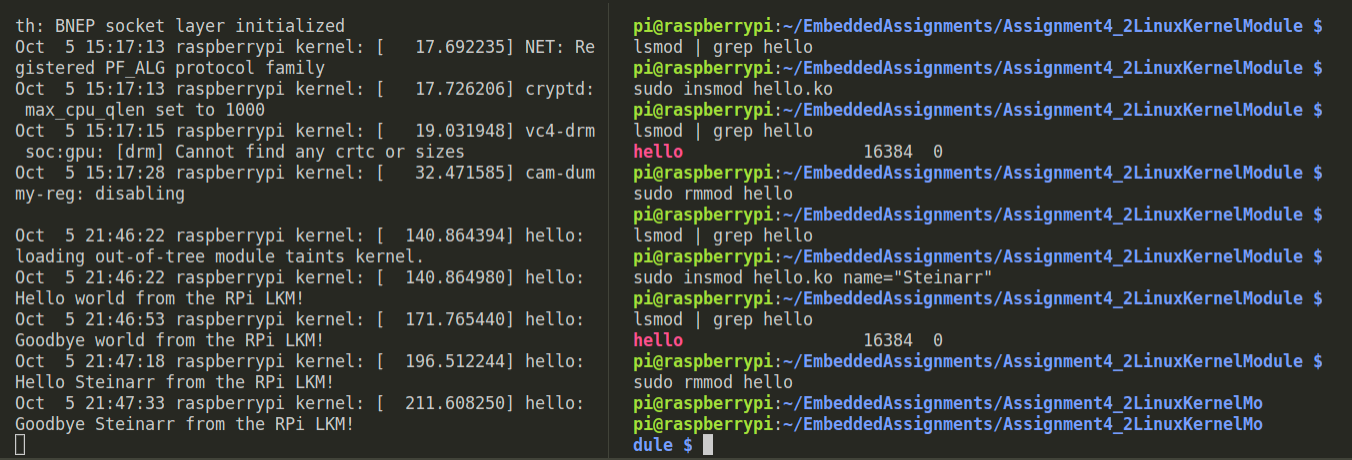
\includegraphics[width=\textwidth]{Assignment4_2LinuxKernelModule/part1_kernel_loading.png}
    \caption{Screenshot of the terminals used to test the loading and unloading of the hello kernel module.}
    \label{fig:kernel_loading}
\end{figure}

\newpage
\section*{Part 2}
The \verb"mydev.c"example given in the assignment was used, it already has the sysfs function \verb!mydev_write()! implemented. \verb!mydev.ko! was compiled with the same Makefile as before and inserted into the kernel. The device node was then created and tested before cleaning up the kernel module and device node.

\begin{figure}[h]
    \centering
    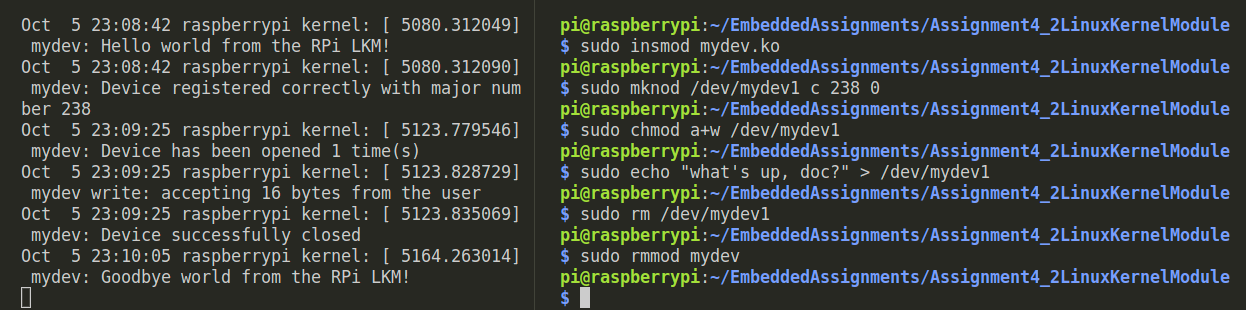
\includegraphics[width=\textwidth]{Assignment4_2LinuxKernelModule/part2_device.png}
    \caption{Screenshot of the terminals used to test the loading and unloading of the mydev device node}
    \label{fig:kernel_loading}
\end{figure}

\section*{Part 3}
A simple application was written that writes an increasing number of characters to \verb!/dev/mydev1!. The program can be seen in Listing \ref{usemydev}

\lstinputlisting[caption={A simple program that writes to the Device Node}]{}\label{usemydev}

\begin{verbatim}[caption={Output of the Kernel Log when use_mydev is run.}]
Oct  6 23:26:25 raspberrypi kernel: [ 2548.997027] mydev:
Device has been opened 4 time(s)
Oct  6 23:26:25 raspberrypi kernel: [ 2548.997070] mydev
write: accepting 1 bytes from the user
Oct  6 23:26:26 raspberrypi kernel: [ 2549.997275] mydev 
write: accepting 2 bytes from the user
Oct  6 23:26:27 raspberrypi kernel: [ 2550.997449] mydev 
write: accepting 3 bytes from the user
Oct  6 23:26:28 raspberrypi kernel: [ 2551.997596] mydev 
write: accepting 4 bytes from the user
Oct  6 23:26:29 raspberrypi kernel: [ 2552.997778] mydev 
write: accepting 5 bytes from the user
Oct  6 23:26:29 raspberrypi kernel: [ 2553.118693] mydev: 
Device successfully closed
\end{verbatim}
\end{document}

